\section{Versuchsaufbau und -durchführung}

\subsection{Versuchsaufbau}

Der allgemeine Versuchsaufbau ist in Abbildung \ref{fig:aufbau_warmepumpe} dargestellt.
An diesem soll die Funktionsweise einer Wärmepumpe erklärt werden.
\begin{figure}
\centering
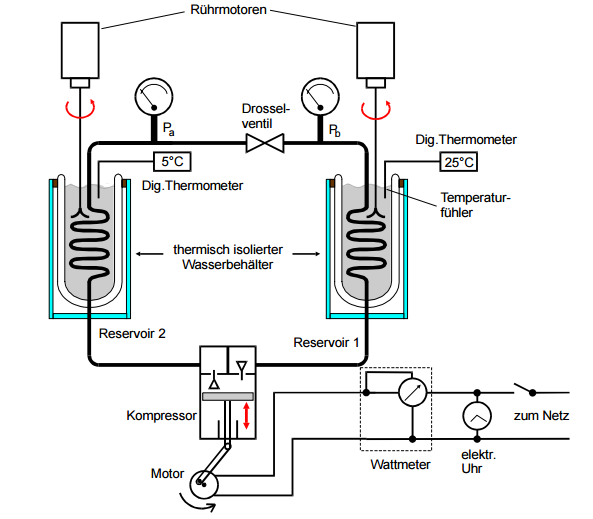
\includegraphics[width=0.9\textwidth]{bilder/versuchsaufbau_1.png}
\caption{Schematischer Aufbau einer Wärmepumpe}
\label{fig:aufbau_warmepumpe}
\end{figure}
Die Wärmepumpe nutzt als Wärmetransportmedium das Gas Dichlodifluormethan.
In Reservoir $1$ wird die Temperatur $T_1$ gemessen, während der Druck $p_b$ wirkt.
Das Gas erreicht es im gasförmigen Zustand. Zu diesem Zeitpunkt ist es
stark erwärmt und so unter Druck komprimiert, dass es sich im Reservoir $1$ wieder verflüssigt.
Während dessen gibt es pro Gramm Gas die Kondensationswärme $L$ in das Reservoir ab.
Dadurch wird dieses aufgeheizt.
Danach fließt das wieder verflüssigte Gas durch einen Reiniger.
Dieser dient dazu, eine blasenfreie Flüssigkeitszufuhr zum anschließenden
Drosselventil zu ermöglichen.
Das Drosselventil dient dazu einen Druckunterschied
$p_b$ - $p_a$ zwischen Reservoir $1$ und $2$ herzustellen.
Es dient aber gleichzeitig auch als Steuervorrichtung.
Denn durch Steuerung des Druckes soll verhindert werden,
dass flüssiges Gas in den Kompressor gelangt.
Nachdem das flüssige Gas das Drosselventil passiert hat,
fließt es in Reservoir $2$. Dort verdampft es und nimmt die Verdampfungswärme
$L$ pro Gramm Substanz auf. Dadurch sinkt die Temperatur des Reservoirs.
Danach gelangt das Gas in den Kompressor. Dieser komprimiert das Gas nahezu adiabatisch.
Dadurch erhöht sich neben der Temperatur des Gases auch der Druck.
Anschließend gelangt es wieder in Reservoir $2$.


\subsection{Versuchsdurchführung}
Zu Beginn des Versuches müssen die beiden Reservoirs mit Wasser gefüllt werden.
Dazu wird mit einem Messkolben die exakte Menge an Wasser ($3$ Liter) eingefüllt.
Danach wird der Kompressor eingeschaltet.
Ab jetzt wird jede Minute die Temperaturen $T_1$ und $T_2$, die Drücke $p_a$ und $p_b$
und die Leistungsaufnahme des Kompressors $A$ abgelesen.
Sobald die Temperatur $T_1$ einen Wert von $50\si{\degreeCelsius}$ erreicht
wird der Kompressor ausgeschaltet.
